\documentclass[11pt, a4paper]{article}

%Preambuła dokumentu
\usepackage{graphicx} 
\usepackage{rotating}
\usepackage{subfigure}
\usepackage{float}
\usepackage{epic}
\usepackage{psfrag}
\usepackage{curves}
\usepackage{listings}
\usepackage{verbatim}
\usepackage{alltt}
\usepackage{fp}
\usepackage{calc}
\usepackage{ifthen}
\usepackage{amssymb}
\usepackage{amsmath}
\usepackage[english]{babel}
\usepackage{geometry}
\usepackage{array}
\usepackage{multirow}
\usepackage{enumerate}
\usepackage{enumitem}
\usepackage[ampersand]{easylist}
\usepackage{changepage}
\usepackage{hyperref}
\usepackage{url}
%\usepackage{parskip}
%\setlength{\parskip}{1ex}
\usepackage[OT4]{fontenc}
\usepackage[utf8]{inputenc} 
\usepackage{color}
\usepackage{xcolor}
\definecolor{bluekeywords}{rgb}{0.13,0.13,1}
\definecolor{greencomments}{rgb}{0,0.5,0}
\definecolor{redstrings}{rgb}{0.9,0,0}

\definecolor{dkgreen}{rgb}{0,0.6,0}
% set the default code style
\lstset{
    frame=tb, % draw a frame at the top and bottom of the code block
    tabsize=4, % tab space width
    showstringspaces=false, % don't mark spaces in strings
    numbers=left, % display line numbers on the left
    commentstyle=\color{greencomments}, % comment color
    keywordstyle=\color{bluekeywords}, % keyword color
    stringstyle=\color{redstrings} % string color
}

% Koniec preambuły dokumentu

% Tekst dokumentu
\begin{document}
\begin{titlepage}

\newcommand{\HRule}{\rule{\linewidth}{0.5mm}} % Defines a new command for the horizontal lines, change thickness here

\center % Center everything on the page
 
%----------------------------------------------------------------------------------------
%	HEADING SECTIONS
%----------------------------------------------------------------------------------------

\textsc{\LARGE Örebro University\\} 
\vspace{0.5cm}
\textsc{\large School of Science and Technology, AASS}\\[0.5cm] % Name of your university/college

%----------------------------------------------------------------------------------------
%	LOGO SECTION
%----------------------------------------------------------------------------------------


\includegraphics[width=4cm]{stuff/orebro_uni_logo}\\[1cm] % Include a department/university logo - this will require the graphicx package

%----------------------------------------------------------------------------------------
%	TITLE SECTION
%----------------------------------------------------------------------------------------

\HRule \\[0.4cm]
{ \huge \bfseries Control of The Velvet Fingers}\\[0.4cm] % Title of your document
\textsc{\large -- Internship final report --}\\[0.5cm] % Minor heading such as course title
\HRule \\[1.5cm]
 
%----------------------------------------------------------------------------------------
%	AUTHOR SECTION
%----------------------------------------------------------------------------------------

\begin{minipage}{0.4\textwidth}
\begin{flushleft} \large
\emph{Author:}\\
\textsc{Kwieciński} Krzysztof % Your name
\end{flushleft}
\end{minipage}
~
\begin{minipage}{0.5\textwidth}
\begin{flushright} \large
\emph{Supervisor:} \\
Dr. Robert \textsc{Krug} % Supervisor's Name
\end{flushright}
\end{minipage}\\[4cm]

% If you don't want a supervisor, uncomment the two lines below and remove the section above
%\Large \emph{Author:}\\
%John \textsc{Smith}\\[3cm] % Your name

%----------------------------------------------------------------------------------------
%	DATE SECTION
%----------------------------------------------------------------------------------------

{\large \today}\\[3cm] % Date, change the \today to a set date if you want to be precise

%----------------------------------------------------------------------------------------
%	LOGO SECTION
%----------------------------------------------------------------------------------------

%\includegraphics{Logo}\\[1cm] % Include a department/university logo - this will require the graphicx package
 
%----------------------------------------------------------------------------------------

\vfill % Fill the rest of the page with whitespace

\end{titlepage}
\tableofcontents
\pagenumbering{gobble}% Remove page numbers (and reset to 1)
\clearpage
\thispagestyle{empty}
\topskip0pt
\vspace*{\fill}
\begin{center} 
  \section*{Abstract} 
\end{center}
In this paper different approaches to control of a gripper are presented. The main focus is on the current (force) control. A gripper used for experiments is \textsf{The Velvet Fingers}, a simple tactile under-actuated gripper.

\begin{figure}[H]
 \begin{center} 
  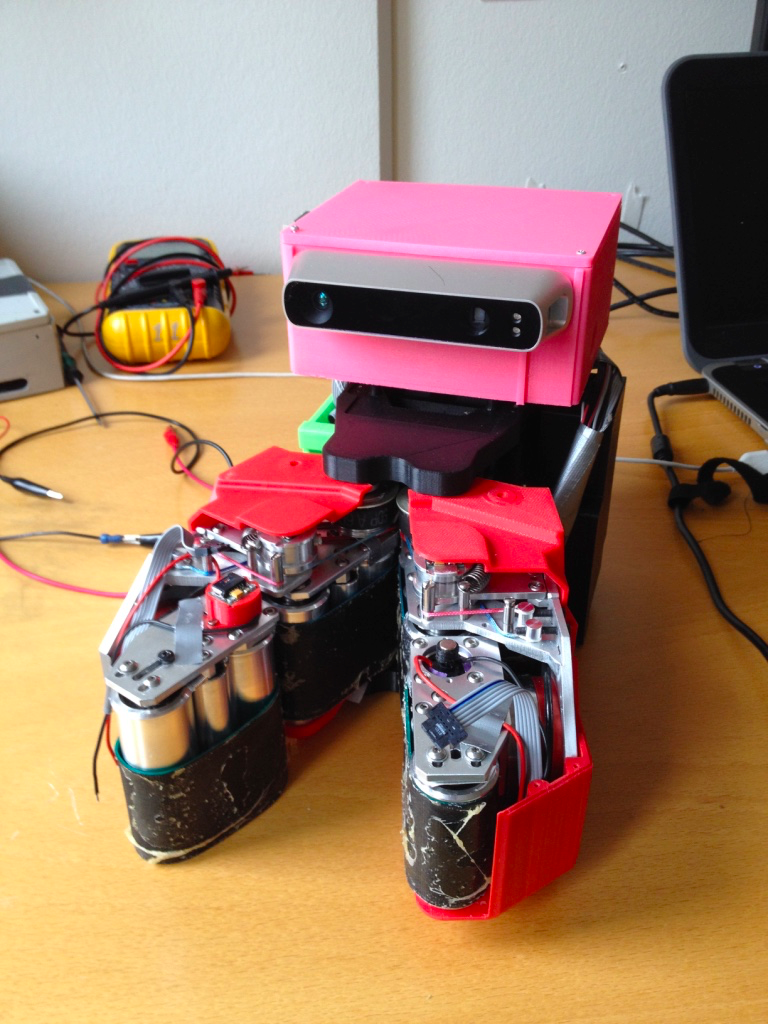
\includegraphics[width=0.4\textwidth]{stuff/my_vfg}
 \end{center}
 \caption{The Velvet Fingers}
 \label{fig:carol_in_house} 
\end{figure}   
\vspace*{\fill}
\clearpage
\pagenumbering{arabic}% Arabic page numbers (and reset to 1)
\section{Introduction}
The report treats of effects of my internship that took place at \textit{School of Science and Technology} at the \textit{Örebro University} in Sweden. I worked for \textit{Centre for Applied Autonomous Sensor Systems}, at the \textit{Mobile Robotics and Olfaction Lab}. A time span I spent here was two months, namely August and September 2015. My main goal was to test different ways of control \textsf{The Velvet Fingers}. Since the gripper is a smart gripper using a novel concept of the end-effector combining simple under-actuated mechanics with high manipulation possibilities, there is only need to control DC motors.
\section{Analysis}
\subsection{DC Armature Model}
A DC motor can be described by two equations:
\begin{equation}
\label{eq:electrical}
	V(t) = L \frac{di(t)}{dt} + Ri(t) + E(t)
\end{equation}
\begin{equation}
\label{eq:mechanical}
	J \dot{\omega}(t) = k_{tau} i(t) - \mu \omega(t) - T_{L}(t),
\end{equation}
where \ref{eq:electrical} describes electrical and \ref{eq:mechanical} describes mechanical aspect of the motor.

It is known that
\begin{equation}
\label{eq:back_emf}
	E(t) = k_{emf} \omega(t),
\end{equation}
\begin{equation}
\label{eq:curr_force}
	T(t) = k_{tau} i(t).
\end{equation}

Combining the above equations and assuming that changes in current are instantaneous yields
\begin{equation}
\label{eq:feedforward_trans}
	V(t) = \frac{R}{k_{tau}} (J \dot{\omega}(t) + \mu \omega(t) + T_{L}(t) ) + k_{emf} \omega(t)
\end{equation}
or simply
\begin{equation}
\label{eq:feedforward_trans_reduced}
	V(t) = Ri(t) + k_{emf} \omega(t)
\end{equation}
if the current is measured. 

Equations \ref{eq:feedforward_trans} and \ref{eq:feedforward_trans_reduced} hold for every state of the motor. However, since we want the gripper to hold an object firmly, desired $\omega$ and $\dot{\omega}$ are zero. That means the final feedforward equation when holding an object can be reduced to
\begin{equation}
\label{eq:feedforward_reduced}
	V(t) = R \frac{T_{L}(t)}{k_{tau}} = R i(t).
\end{equation}

Nomenclature:
$R$ - motor terminal resistance,
$L$ - motor terminal inductance,
$i$ - current,
$E$ - back electromotive force,
$J$ - rotor inertia moment,
$\omega$ - rotor angular velocity,
$\dot{\omega}$ - rotor angular acceleration,
$k_{tau}$ - torque constant,
$k_{emf}$ - speed constant,
$T_{L}$ - load torque.  
\section{Implementation}
\subsection{Matlab}
The first step was to understand the working principle of a DC motor. After getting such knowledge, I had to verify it in Matlab and Simulink. I created two models of a DC motor in Simulink: one built of only basic blocks and second using blocks from the Simscape library. Models are shown on figures \ref{fig:basic} and \ref{fig:hbridge}.

\begin{figure}%[H]
 \begin{center} 
  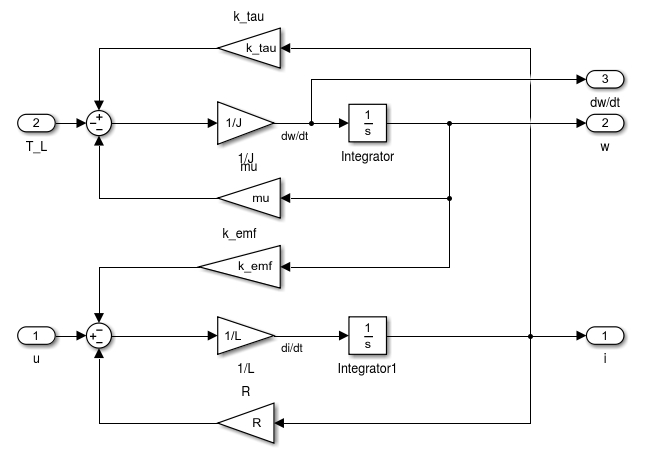
\includegraphics[width=0.7\textwidth]{./stuff/basic_blocks}
 \end{center}
 \caption{A model of a DC motor in Simulink built of basic blocks}
 \label{fig:basic} 
\end{figure}   

\begin{figure}%[H]
 \begin{center} 
  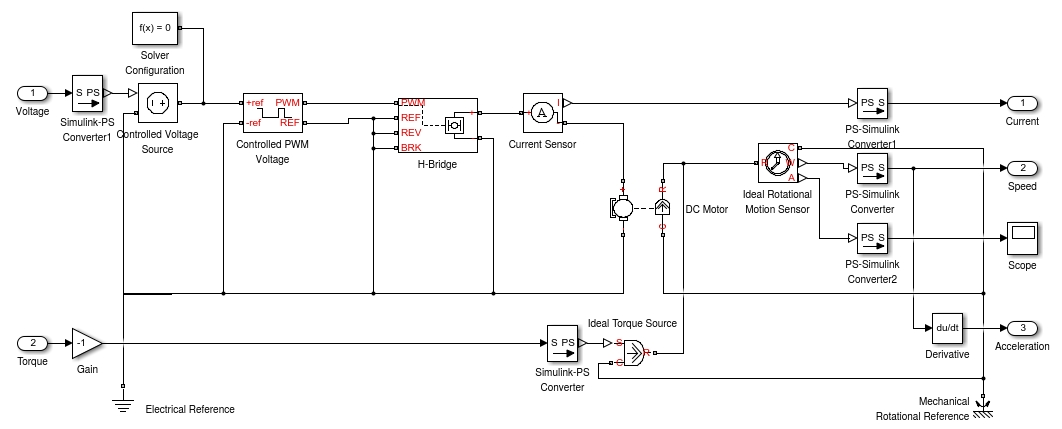
\includegraphics[width=\textwidth]{./stuff/simscape}
 \end{center}
 \caption{A model of a DC Motor in Simulink built of blocks from the Simscape library}
 \label{fig:hbridge} 
\end{figure}   

I tested both models using scripts written in Matlab. Inputs of the system were voltage and applied force, and outputs were current, angular velocity and acceleration. Tests were done for open and closed loop. Control of the process variable was done with a PID controller. Results for both models were almost identical and the simulations confirmed theoretical knowledge and developed my intuition.

\begin{figure}%[H]
 \begin{center} 
  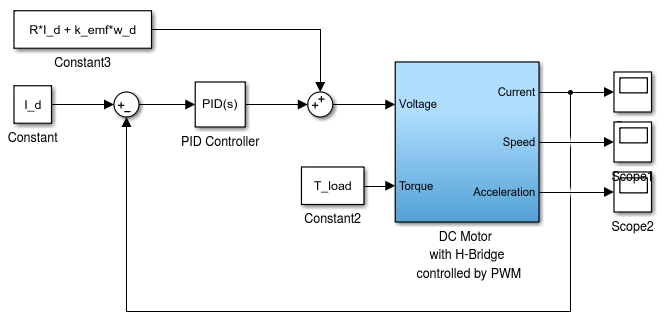
\includegraphics[width=0.7\textwidth]{./stuff/control_loop}
 \end{center}
 \caption{An example control loop with feedforward term}
 \label{fig:loop} 
\end{figure} 

\subsection{Arduino}
Afer getting some experience, I started working with hardware. The computations and control were done by \textsf{Arduino Due} board. The code was written in \textsf{C++}. With such combination, I was able to write a program containing a lot of operations using a high-level programming language.

Control of speed and direction of the motor's movement was done with use of an external H-Bridge and a PWM signal from \textsf{Arduino}.

Arduino was connected with a computer through a serial port. As a middleware \textsf{The Robot Operating System} was used. \textsf{ROS} allowed to change parameters on-line and provided opportunity to observe and visualize values of chosen variables.

Thanks to usage of encoders and measuring the current flowing through the motor, I was able to implement various types of control, for instance:
\begin{itemize}
	\item current (force) control,
	\item position control,
	\item velocity control,
	\item stiffness control,
	\item impedance control,
	\item parallel force/position control.
\end{itemize}  

Because the control was dedicated for a gripper, the most important was the first one.

\subsection{Documentation}
All files with a detailed documentation of the code generated by \textsf{Doxygen} are available at the \textsf{GitHub} repository.
\section{Case studies}
For conducting experiments two setups were used. A basic one consisted only from one DC motor. The second was \textsf{The Velvet Fingers}.

\subsection{Basic methods}
Three fundamental methods of control are: current, position and velocity control. They all rely on measuring one process variable (PV) and try to reach the setpoint (SP) with use of a PID controller, which output is the control variable (CV).

\begin{equation}
u(t) = K_p e(t) + K_i \int_{0}^{t}e(\tau)d\tau + K_d \frac{de}{dt} 
\end{equation}

\subsubsection{Current Control}
Current control can be identified with force control. Even though there are no tactile sensors, hence the force is not explicitly measured, the  applied force can be implicitly calculated from \ref{eq:curr_force}. 

\begin{figure}%[H]
 \begin{center} 
  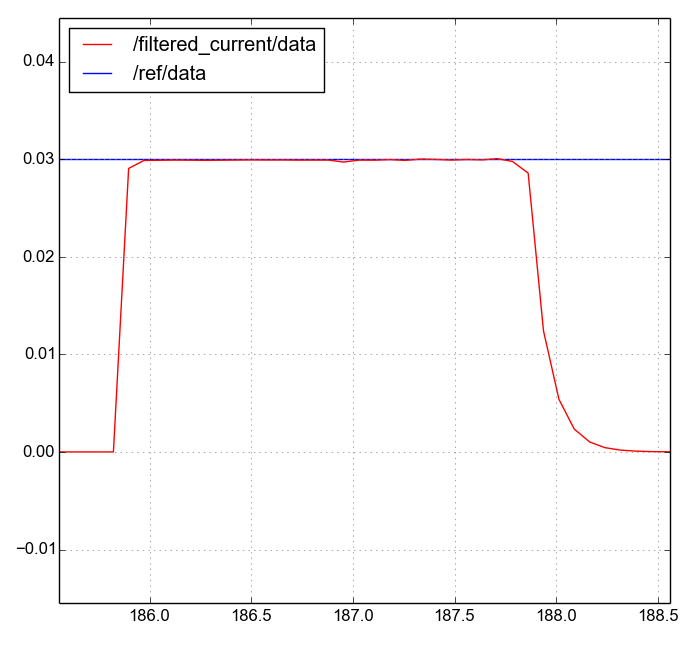
\includegraphics[width=0.55\textwidth]{./stuff/filtered_current}
 \end{center}
 \caption{An exaple plot of the current control}
 \label{fig:current_plot} 
\end{figure}   

Figure \ref{fig:current_plot} presents changes of current flowing through the motor in time. X-axis is time [s], Y-axis is current [A]. We can see three phases: in the beginning and the end the motor was running without any constraints, in the middle phase the movement was constrained.
The response was almost instantaneous, and the control variable reached the setpoint very precisely and without oscillations. 

\subsubsection{Position Control}
\begin{figure}%[H]
 \begin{center} 
  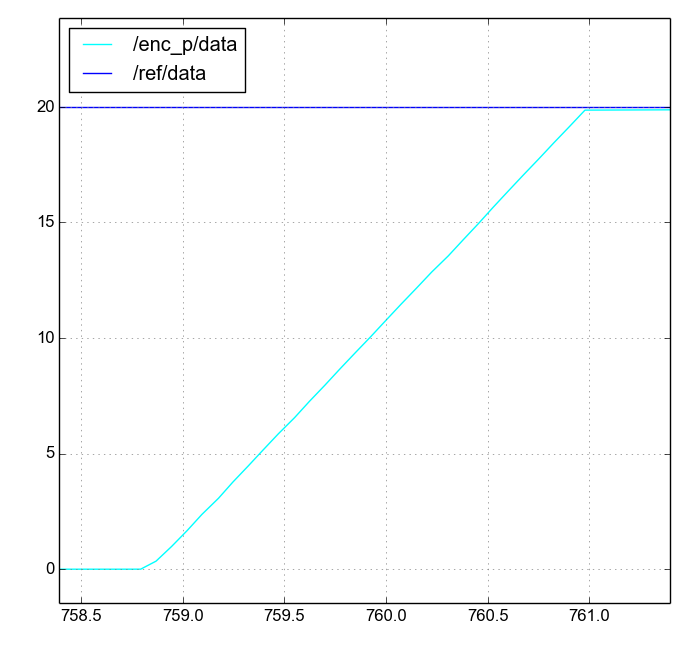
\includegraphics[width=0.55\textwidth]{./stuff/enc_p_plot}
 \end{center}
 \caption{An exaple plot of the position control}
 \label{fig:position_plot} 
\end{figure} 

Figure \ref{fig:position_plot} presents changes of the motor's position in time. X-axis is time [s], Y-axis is position [rad]. After applying the voltage the movement was steady.
The control variable reached the setpoint very precise and without oscillations.

\subsubsection{Velocity Control}
\begin{figure}%[H]
 \begin{center} 
  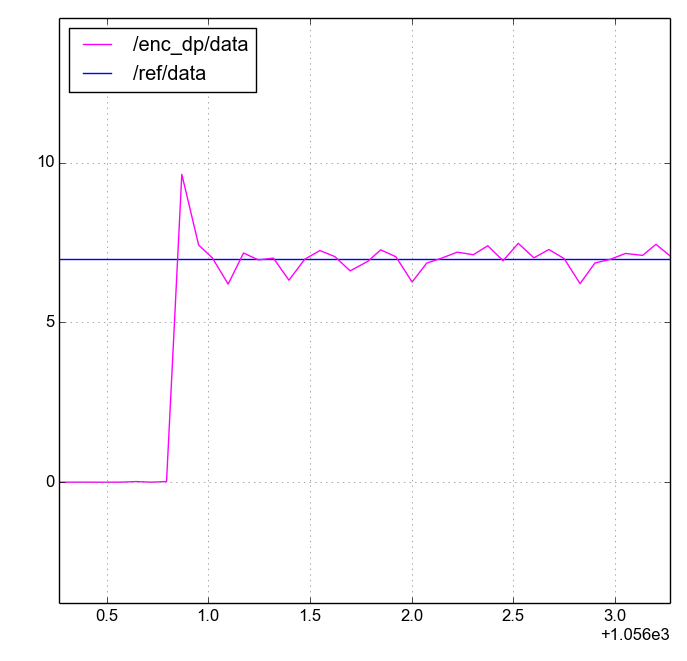
\includegraphics[width=0.55\textwidth]{./stuff/enc_dp_plot}
 \end{center}
 \caption{An exaple plot of the velocity control}
 \label{fig:velocity_plot} 
\end{figure} 

Figure \ref{fig:velocity_plot} presents changes of the motor's velocity in time. X-axis is time [s], Y-axis is angular velocity [rad/s]. After applying the voltage the motor reached the setpoint very fast. Although oscillations are presented in the plot, the movement of the motor was actually smooth. The oscillations are visible due to measurements done by encoder and derivating the position, which introduce some noise.

\subsection{Complex methods}
When interacting with the environment, there is need for more sophisticated methods. The control variable is calculated based on two or more process variables.

Nomenclature: $p$ - current position, $\dot{p}$ - current velocity, $\ddot{p}$ - current acceleration, $f$ - current force, $_d$ - desired value, $K_p$ - position coefficient, $K_v$ - velocity coefficient, $K_f$ - force coefficient, $K_i$ - integral coefficient, $M$ - mass, $B$ - damping, $K$ - stiffness.

\subsubsection{Stiffness Control}
Stiffness control derives from a position control scheme of PD type.

\begin{equation}
u(t) = K_{p}(p_{d} - p) - K_{v} \dot{p},
\end{equation}

\begin{figure}%[H]
 \begin{center} 
  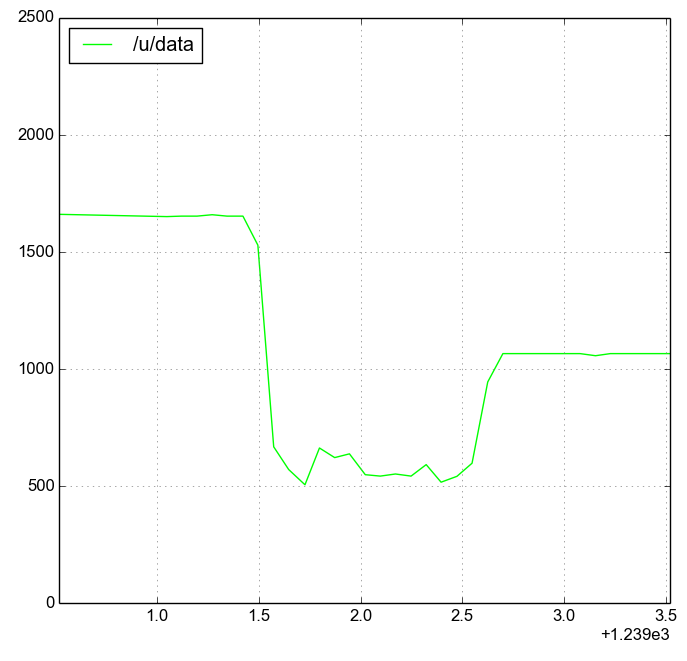
\includegraphics[width=0.55\textwidth]{./stuff/stiffness_plot}
 \end{center}
 \caption{An exaple plot of the stiffness control}
 \label{fig:stiffness_plot} 
\end{figure} 

Figure \ref{fig:stiffness_plot} presents changes of the control variable in time. X-axis is time [s], Y-axis is the CV. We can see three phases: in the beginning and the end the movement is constrained, in the middle phase the motor is running without any constraints.
When in contact with the environment, the CV is steady and larger than during the unconstrained motion.
Since stiffness control derives from a position control, the closer to the setpoint, the lower the CV. 

\subsubsection{Impedance Control}
In impedance control the input is flow (velocity or displacement) and the output is effort (force).
In directions where the robot has to be environment-sensitive, impedance is low, otherwise impedance is high. The desired impedance behavior is a trade-off between trajectory error and force error. If the motion is unconstrained, force will be zero and the robot will move to the reference position. 

\begin{equation}
u(t) = M(\ddot{p}_d - \ddot{p}) + B(\dot{p}_d-\dot{p}) + K(p_d-p) - K_f f
\end{equation}

Desired acceleration and velocity are usually not present to guarantee passivity when in contact with the environment.

\begin{figure}%[H]
 \begin{center} 
  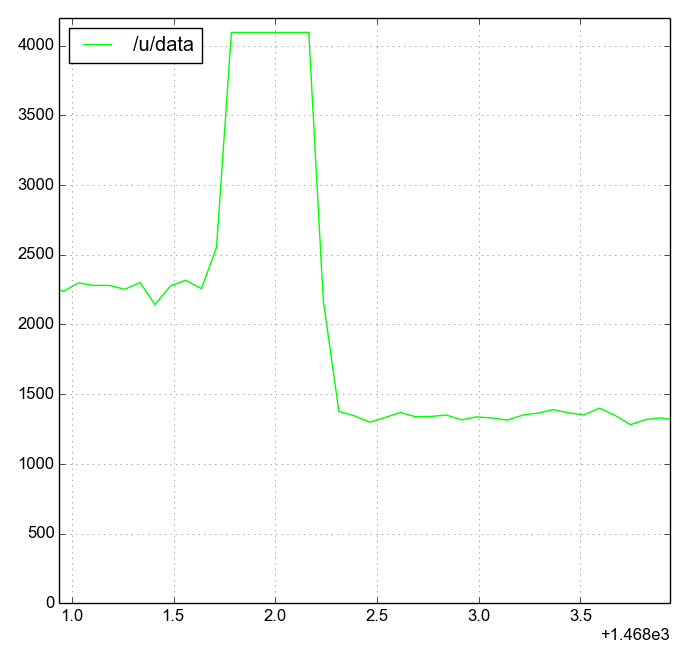
\includegraphics[width=0.55\textwidth]{./stuff/impedance_plot}
 \end{center}
 \caption{An exaple plot of the impedance control}
 \label{fig:impedance_plot} 
\end{figure} 

Figure \ref{fig:impedance_plot} presents changes of the control variable in time. X-axis is time [s], Y-axis is the CV. We can see three phases: in the beginning and the end the movement is constrained, in the middle phase the motor is running without any constraints.
When in contact with the environment, the CV is steady and smaller than during the unconstrained motion.
Such behaviour keeps the interaction force in desired boundaries and guarantees reaching the setpoint, if possible.
 
\subsubsection{Parallel Force/Position Control}
In order to combine features of stiffness control and force control, a parallel force/position regulator can be designed where a PI force control action plus desired force feedforward is used in parallel to a PD position control action.
The position controller is an impedance while the force controller results in a filtering action on the force variables.
 
\begin{equation}
u(t) = M \ddot{e}_p +  K_{v} \dot{e}_p + K_p e_p + K_f e_f + K_i\int_{0}^{t} e_f d\tau,
\end{equation}
where error $e$
\begin{equation}
e_{variable}(t) = variable_{desired} - variable(t).
\end{equation}

\begin{figure}%[H]
 \begin{center} 
  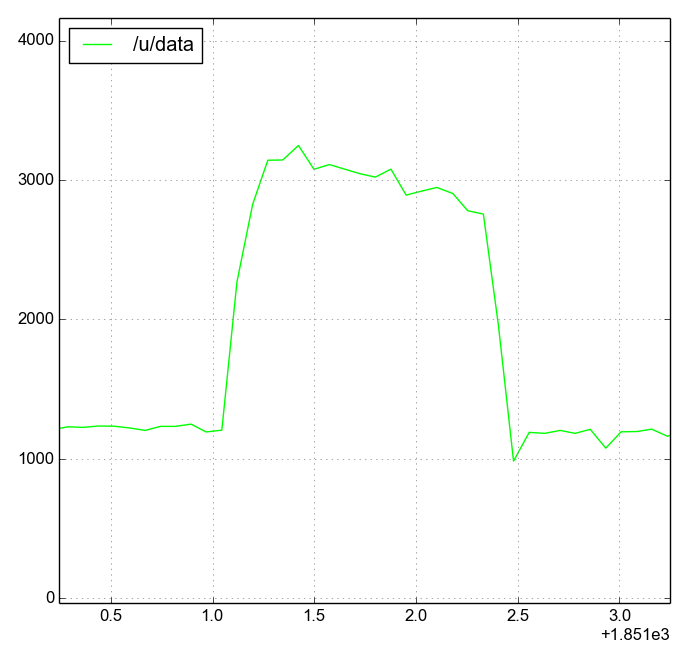
\includegraphics[width=0.55\textwidth]{./stuff/force_pos_plot}
 \end{center}
 \caption{An exaple plot of the parallel force/position control}
 \label{fig:force_pos_plot} 
\end{figure} 

Figure \ref{fig:force_pos_plot} presents changes of the control variable in time. X-axis is time [s], Y-axis is the CV. We can see three phases: in the beginning and the end the movement is constrained, in the middle phase the motor is running without any constraints.
When in contact with the environment, the CV is steady and smaller than during the unconstrained motion. When moving freely and going in direction of the setpoint, the CV slowly decreases.
Such behaviour keeps the interaction force at desired level independently of the position error and guarantees reaching the setpoint, if possible. 
\section{Conclusion}
There are plenty of methods to control a DC motor. In this report a couple of them were treated. 

Working with the environment requires interaction so taking into consideration more than one variable is necessary. The most obvious conclusion is that the more complicated type of control, the more effort is needed to achieve the goal. It is why all the basic methods always worked fast and reliable, and the more complex did not. The problem is achieving two different goals which is practically impossible. All things considered make more complex methods more difficult to implement, however, if properly done, they are the best choice. The point is to find a fair trade-off between goals that should be achieved. 

Furthermore, working with hardware might be a source of difficult to track down problems. Due to working with not impeccable measuring equipment, filtering variables, i.e. current and position, is really important. A PID controller plays a crucial role in control. If properly tuned, the controller is fast and precise. 

Future research efforts will be devoted to improving all types of control.
 

\newpage
\bibliographystyle{abbrv}
\nocite{*}
\bibliography{bibliography} 

\end{document}